\documentclass[a4paper, top=10mm]{article}
%for writing from the top
\usepackage{fullpage}
%for math
\usepackage{amsmath}
\usepackage{mathrsfs}
\usepackage{amsthm}
\usepackage{amsfonts}
%for images
\usepackage{graphicx}
%for color
\usepackage{xcolor}
%for title
\title{\textbf{\huge{Bug in Borwein Integrals}}}
\author{Enigma n\textsuperscript{o}3}
\date{2\textsuperscript{nd} December 2022}

\newtheorem*{hint}{Hint}

\addtolength{\voffset}{-2cm}
\addtolength{\textheight}{5cm}


\begin{document}
	\maketitle
	
	Looking at th first few cases, it seems that
	$
	\int_{-\infty}^{+\infty} \prod_{k=0}^{n} \frac{\sin(x/(2k+1)}{x/(2k+1)} dx = \pi
	$
	for all $n \in \mathbb{N}$.
	
	It is in fact true that:
	$$
	\int_{-\infty}^{+\infty} \frac{\sin(x)}{x} dx = \pi
	$$
	$$
	\int_{-\infty}^{+\infty} \frac{\sin(x)}{x}\frac{\sin(x/3)}{x/3} dx = \pi
	$$
	$$
	\int_{-\infty}^{+\infty} \frac{\sin(x)}{x}\frac{\sin(x/3)}{x/3}\frac{\sin(x/5)}{x/5} dx = \pi
	$$
	
	However, it will eventually fail:
	$$
	\int_{-\infty}^{+\infty} \prod_{k=0}^{100} \frac{\sin(x/(2k+1)}{x/(2k+1)} dx \neq \pi
	$$

	\vspace{1cm}

	\begin{center}
		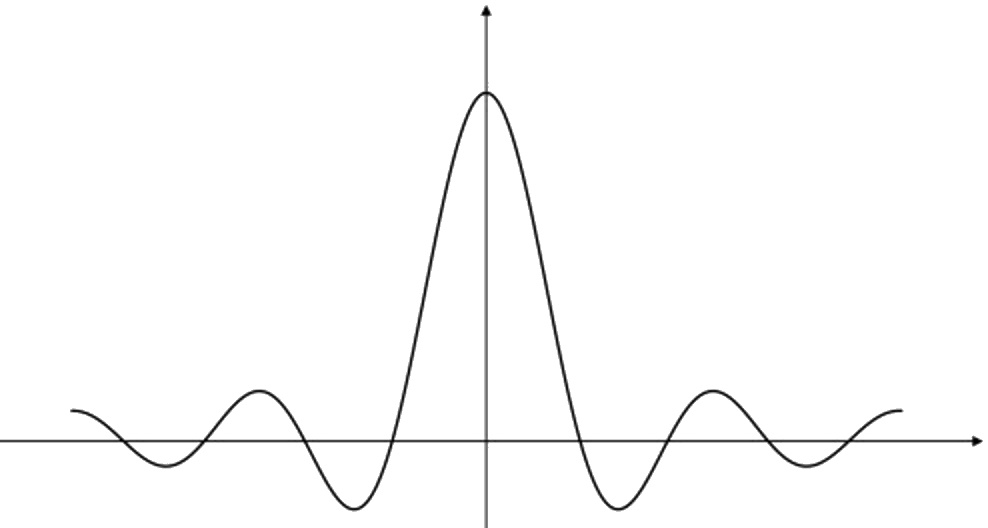
\includegraphics[height=200pt]{03sinc_plot.jpg}\\
		Plot of $\frac{\sin(x)}{x}$
	\end{center}

	\vspace{3cm}
	
	\textbf{What is the first $n \in \mathbb{N}$ such that 
	$
	\int_{-\infty}^{+\infty} \prod_{k=0}^{n} \frac{\sin(x/(2k+1)}{x/(2k+1)} dx \neq \pi
	$
	?}
	
\end{document}